\chapter{VLANs and Subnetting}

\thispagestyle{standard}
\pagestyle{standard}

The given network was a 192.168.1.0/24 network, which had to be divided into 4 subnets. Each subnet had its own \ac{VLAN}.

\begin{table}[h]
\centering
\begin{tabular}{r||r|r|r|r|}
\textbf{VLAN} & \textbf{Hosts} & \textbf{Network ID/Subnet} & \textbf{First usable IP} & \textbf{Broadcast IP} \\

		\hline
10 & 120 & 192.168.1.0/25 & 192.168.1.1 & 192.168.1.127  \\
20 & 60 & 192.168.1.128/26 & 192.168.1.129 & 192.168.1.191  \\
30 & 30 & 192.168.1.192/27 & 192.168.1.193 & 192.168.1.223  \\
99 & 10 & 192.168.1.224/28 & 192.168.1.224 & 192.168.1.239  \\

\end{tabular}
\caption{VLANs and Subnets}
\label{tab:vlan_subnets}
\end{table}

The final subnetting that was used in the lab can be seen in table  \ref{tab:vlan_subnets}.

The first usable IP address in each subnet was given to the router to that subnet.

\chapter{Topology}

The following topology (Figure \ref{img:topo}, taken from the Moodle instructions, had to be recreated in the lab.

\begin{figure}[H]
	\centering
	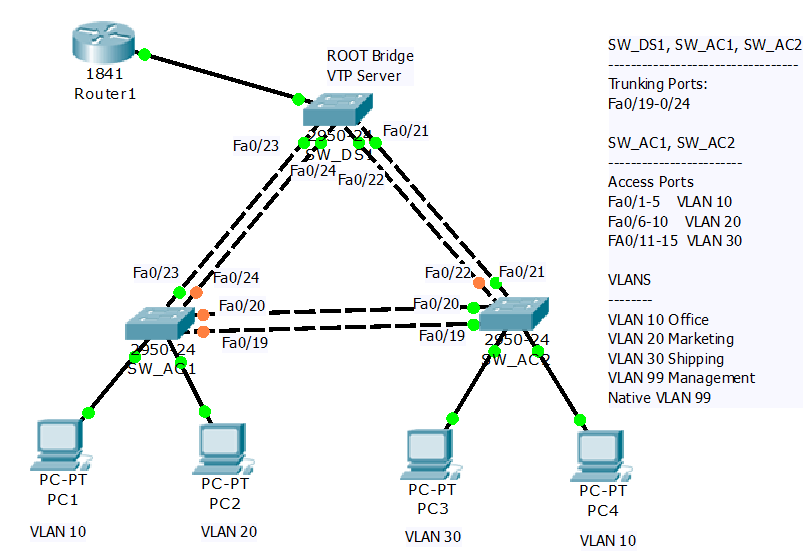
\includegraphics[width=0.9\textwidth]{img/topo.png}
	\caption{Topology (Moodle)}
	\label{img:topo}
\end{figure}

\section{Basic configuration}

Each device was configured with basic settings like Hostname, \ac{MOTD} and a password.

\lstset{escapeinside={\%*}{*)},numbers=left}%oder numbers=left
\begin{lstlisting}[caption={Basic configuration},label={lst:debug_s3},language={}]
enable
conf terminal
hostname SW_AC1
banner motd # Unauthorized access prohibited! #
enable secret cisco
service password-encryption
\end{lstlisting}

These few lines would set hostname and the \ac{MOTD} and encrypt the configured password `cisco'.

These settings were applied onto every device, with the hostname changed.

\section{Spanning Tree}

The use of the \ac{STP} allows to detect loops in the network and creates a first redundancy layer. \ac{STP} uses a tree structure in which every Switch (bridge) in the network knows the best path to the root bridge. Redundant paths to the root bridge will be blocked for normal traffic.

\texttt{SW\_DS1} had to be configured as root bridge.

\lstset{escapeinside={\%*}{*)},numbers=left}%oder numbers=left
\begin{lstlisting}[caption={\ac{STP} configuration root},label={lst:stp},language={}]
conf terminal
spanning-tree mode pvst
spanning-tree vlan 1,10,20,30,99 priority 4096
\end{lstlisting}

This is the configuration for the root bridge. The bridge with the lowest bridge ID will become root bridge. In this configuration the ID is \texttt{4096}, the other switches in the network have been set to a higher bridge ID to ensure that \texttt{SW\_DS1} becomes root.

The \ac{PVST} mode has been used to spawn a \ac{STP} instance per VLAN. This would allow to load balance certain \ac{VLAN}s to different paths, but this was not used in this lab. The \ac{PVST} mode was used for all configured \ac{VLAN}s.

\chapter{VTP}

The \ac{VTP} allows the distribution of configured \ac{VLAN}s to all switches in the VTP domain. This allows easier reconfiguration of VLANs. For this one switch has to act as the VTP server, while the other ones get the configuration from the server.

Similar to the STP root bridge, \texttt{SW\_DS1} had to be configured as \ac{VTP} server.

\lstset{escapeinside={\%*}{*)},numbers=left}%oder numbers=left
\begin{lstlisting}[caption={\ac{VTP} and VLAN},label={lst:vtps},language={}]
vlan 10 name Office
vlan 20 name Marketing
vlan 30 name Shipping
vlan 99 name Management

vtp mode server
vtp version 2
vtp lab
vtp cisco
\end{lstlisting}

Those commands created the 4 \ac{VLAN}s and the \ac{VTP} server on \texttt{SW\_DS1}.

Version 2 had to be used, as we encountered some problems with \ac{VTP} version 3.
\\


The client configuration for the switches can be seen in \ref{lst:vtps}.

\lstset{escapeinside={\%*}{*)},numbers=left}%oder numbers=left
\begin{lstlisting}[caption={\ac{VTP} client},label={lst:vtps},language={}]
vtp mode client
vtp version 2
vtp lab
vtp cisco
\end{lstlisting}

\chapter{\ac{VLAN} setup}

In this chapter, the ports on the switch had to be configured as either VLAN access ports, or trunk ports for the uplinks to the other switches.

The assignment from VLAN to port can be seen in table \ref{tab:vlan_ports}.

\begin{table}[h]
\centering
\begin{tabular}{r||r}
\textbf{Ports} & \textbf{VLANs}  \\

		\hline
Fa0/1-5 & 10 \\
Fa0/6-10 & 20 \\
Fa0/11-15 & 30    \\
Fa0/19-24 & Trunk ports  \\
everything else & 1

\end{tabular}
\caption{VLANs to ports}
\label{tab:vlan_ports}
\end{table}

\lstset{escapeinside={\%*}{*)},numbers=left}%oder numbers=left
\begin{lstlisting}[caption={Access port configuration},label={lst:accport},language={}]
int range fa0/1 - 5
switchport mode access
switchport access vlan 10
\end{lstlisting}

The commands in \ref{lst:accport} have been adapted for the different VLANs.
The access ports have been configured on both \texttt{SW\_AC1} and \texttt{SW\_AC2}.

\lstset{escapeinside={\%*}{*)},numbers=left}%oder numbers=left
\begin{lstlisting}[caption={Trunk port configuration},label={lst:accport},language={}]
int fa0/21
switchport mode trunk
switchport trunk allowed vlan 10,20,30,99
switchport trunk native vlan 99
\end{lstlisting}

The native VLAN is 99, which is also the management VLAN, which may not be wise from a security point of view. The native VLAN will not be tagged (802.1Q) when transmitted through the trunk port. For ease of configuration some unused ports where assigned to the Management VLAN.

To test this configuration we put a PC in each VLAN on each switch and used the `ping' tool, which showed a successful configuration.

% ausgabe einf�gen?

\chapter{Inter-VLAN Routing}

To make communication between the VLANs possible a router needs to be used. The router has an IP address (see table \ref{tab:vlan_subnets}) in each subnet. All PCs can therefore reach the router.

\lstset{escapeinside={\%*}{*)},numbers=left}%oder numbers=left
\begin{lstlisting}[caption={Router configuration},label={lst:routervlan},language={}]
conf terminal
int Gig0/0.10
encapsulation dot1q 10
ip address 192.168.1.1 255.255.255.128
\end{lstlisting}

The commands in listing \ref{lst:routervlan} will create a subinterface on gig0/1 and set the encapsulation to the IEEE 802.1Q standard. Then an IP address is assigned to that interface. This commands have been adopted for every VLAN.

For the native VLAN, the encapsulation line had been changed to:

\texttt{encapsulation dot1Q 99 native}

to mark VLAN 99 as the native VLAN.